\chapter{Implementierung}
\label{impl}

\section{Überblick}

Um ein System wie in \ref{ziele} beschrieben zu entwickeln, muss zunächst ein Algorithmus festgelegt werden, der die gewünschten Eigenschaften hat. Dieser Algorithmus wird den Kern des Systems bilden. In \ref{algo} wird diese Entscheidung erläutert. Dann wird in \ref{sprache} die Wahl der Programmiersprache erklärt und in \ref{konzept} auf die grundlegenden Konzepte des zu entwickelnden Systems eingegangen.

\subsection{Wahl des Algorithmus}
\label{algo}

Die Kandidaten sind die in \ref{algos} vorgestellten Algorithmen Paxos, Zab und Raft. Die Beschreibung von Paxos ist sehr theoretisch und nicht praxisnah gehalten, was zu Problemen bei der Implementierung führen könnte, die nicht im Dokument beschrieben sind und für die somit zeitaufwändig eigene Lösungen entworfen werden müssten. Dies bestätigen die wenigen Paxos-Implementierungen und die Berichte von Autoren, die auf Paxos basierende Systeme entwickelt haben und von Schwierigkeiten bei der Implementierung berichten. Zab wurde speziell für Zookeeper entwickelt und wurde soweit bekannt in keinem anderen System implementiert. 

Die Beschreibung von Raft ist sehr praxisnah und es wird auf viele Implementierungsdetails eingegangen. Außerdem sind bereits einige Implementierungen vorhanden, was darauf schließen lässt, dass Raft einfacher zu implementieren ist als Paxos. Die Autoren von Zab erklären, dass ein Vorteil von ihrem System gegenüber Paxos ist, dass nebenläufige Anfragen von Clients die Reihenfolge nicht ändern können, und zeigen mit einem Beispiel, dass dies bei Paxos der Fall sein kann. Da Raft ebenfalls auf dem Replicated-State-Machine-Modell basiert, können hier ebenso die Client-Anfragen von einem Leader beliebig geordnet werden. Dies sollte jedoch in der Praxis kein Problem darstellen: Bei Anfragen von verschiedenen Clients kann vorher keine Reihenfolge bestimmt werden. Bei mehreren gleichzeitigen Anfragen von einem Client kann dieser eine Reihenfolge festlegen. Dann kann über ein Netzwerk-Protokoll mit Sequenznummern (wie z.B. TCP) sichergestellt werden, dass diese bei jedem Raft-Leader in dieser Reihenfolge ankommen. Dadurch ist sicher, dass die Anfragen auch in dieser Reihenfolge vom System bearbeitet werden.
 
Aus den genannten Gründen wurde Raft als Algorithmus für das zu entwickelnde System ausgewählt.

\subsection{Wahl der Programmiersprache}
 \label{sprache}

Als Programmiersprache für das zu entwickelnde System wurde Java gewählt. Java ist eine in der Industrie weit verbreitete Sprache, für die es viele gut entwickelte Tools und Bibliotheken gibt. Ein Vorteil gegenüber dynamischen Programmiersprachen wie Python ist auch die Typsicherheit, die bereits zur Compilezeit sichergestellt wird. Dies kann bei der Erkennung von subtilen Fehlern im Code helfen, was bei eher komplexeren Systemen wie einem Einigungsalgorithmus wichtig ist. Außerdem erleichtert die Wahl von Java die vorgesehene Integration in DXRAM, da DXRAM ebenfalls in Java implementiert ist. Für das Build-Management wird Gradle verwendet.

\subsection{Konzept der Implementierung}
 \label{konzept}

Da das System in DXRAM verwendet werden soll, speziell dafür entwickelt wird und Raft als Einigungsalgorithmus nutzen wird, soll das System \textbf{DXRaft} heißen. Die Implementierung soll möglichst performant sein und später Möglichkeiten zur Optimierung bieten. Dazu ist es sinnvoll, sie möglichst leichtgewichtig zu gestalten und keine großen Frameworks oder Bibliotheken zu verwenden. Außerdem soll die Nutzung möglichst einfach sein. Insbesondere sollte das Bootstrapping möglichst automatisch ablaufen können, sodass der Einsatz in einem verteilten System keine zusätzlichen Tools benötigt.

Das System besteht aus Server-Instanzen und Clients. Die Server-Instanzen bilden ein Cluster und führen den Einigungsalgorithmus aus. Die Clients verbinden sich mit dem Cluster und bieten dem Nutzer eine Schnittstelle zum System an. Server und Clients sollen sowohl Standalone als auch als Bibliothek genutzt werden können. Das Nutzen als Bibliothek hat den Vorteil, dass für das System kein eigener Prozess gestartet werden muss. Abbildung \ref{fig:components} zeigt ein Beispiel, wie die Nutzung von DXRaft aussehen kann: Auf ausgewählten Knoten werden DXRaft-Server-Instanzen gestartet. Diese bilden den Cluster, welches den Raft-Algorithmus ausführt. Auf allen anderen Knoten werden Clients genutzt, die die Anfragen an den Cluster weiterleiten. Da die Anfragen alle vom Leader bearbeitet müssen, senden die Clients die Anfragen direkt an den Leader, um die Anfragen möglichst schnell zu bearbeiten. Später könnte noch die Möglichkeit eingebaut werden, dass Clients die Anfragen nicht direkt an den Leader senden, um diesen nicht zu überfordern. Sie könnten sie z.B. auch zunächst an einen Follower senden, der die Anfrage dann an den Leader weiterleitet.

\begin{figure}[h]
	\centering
	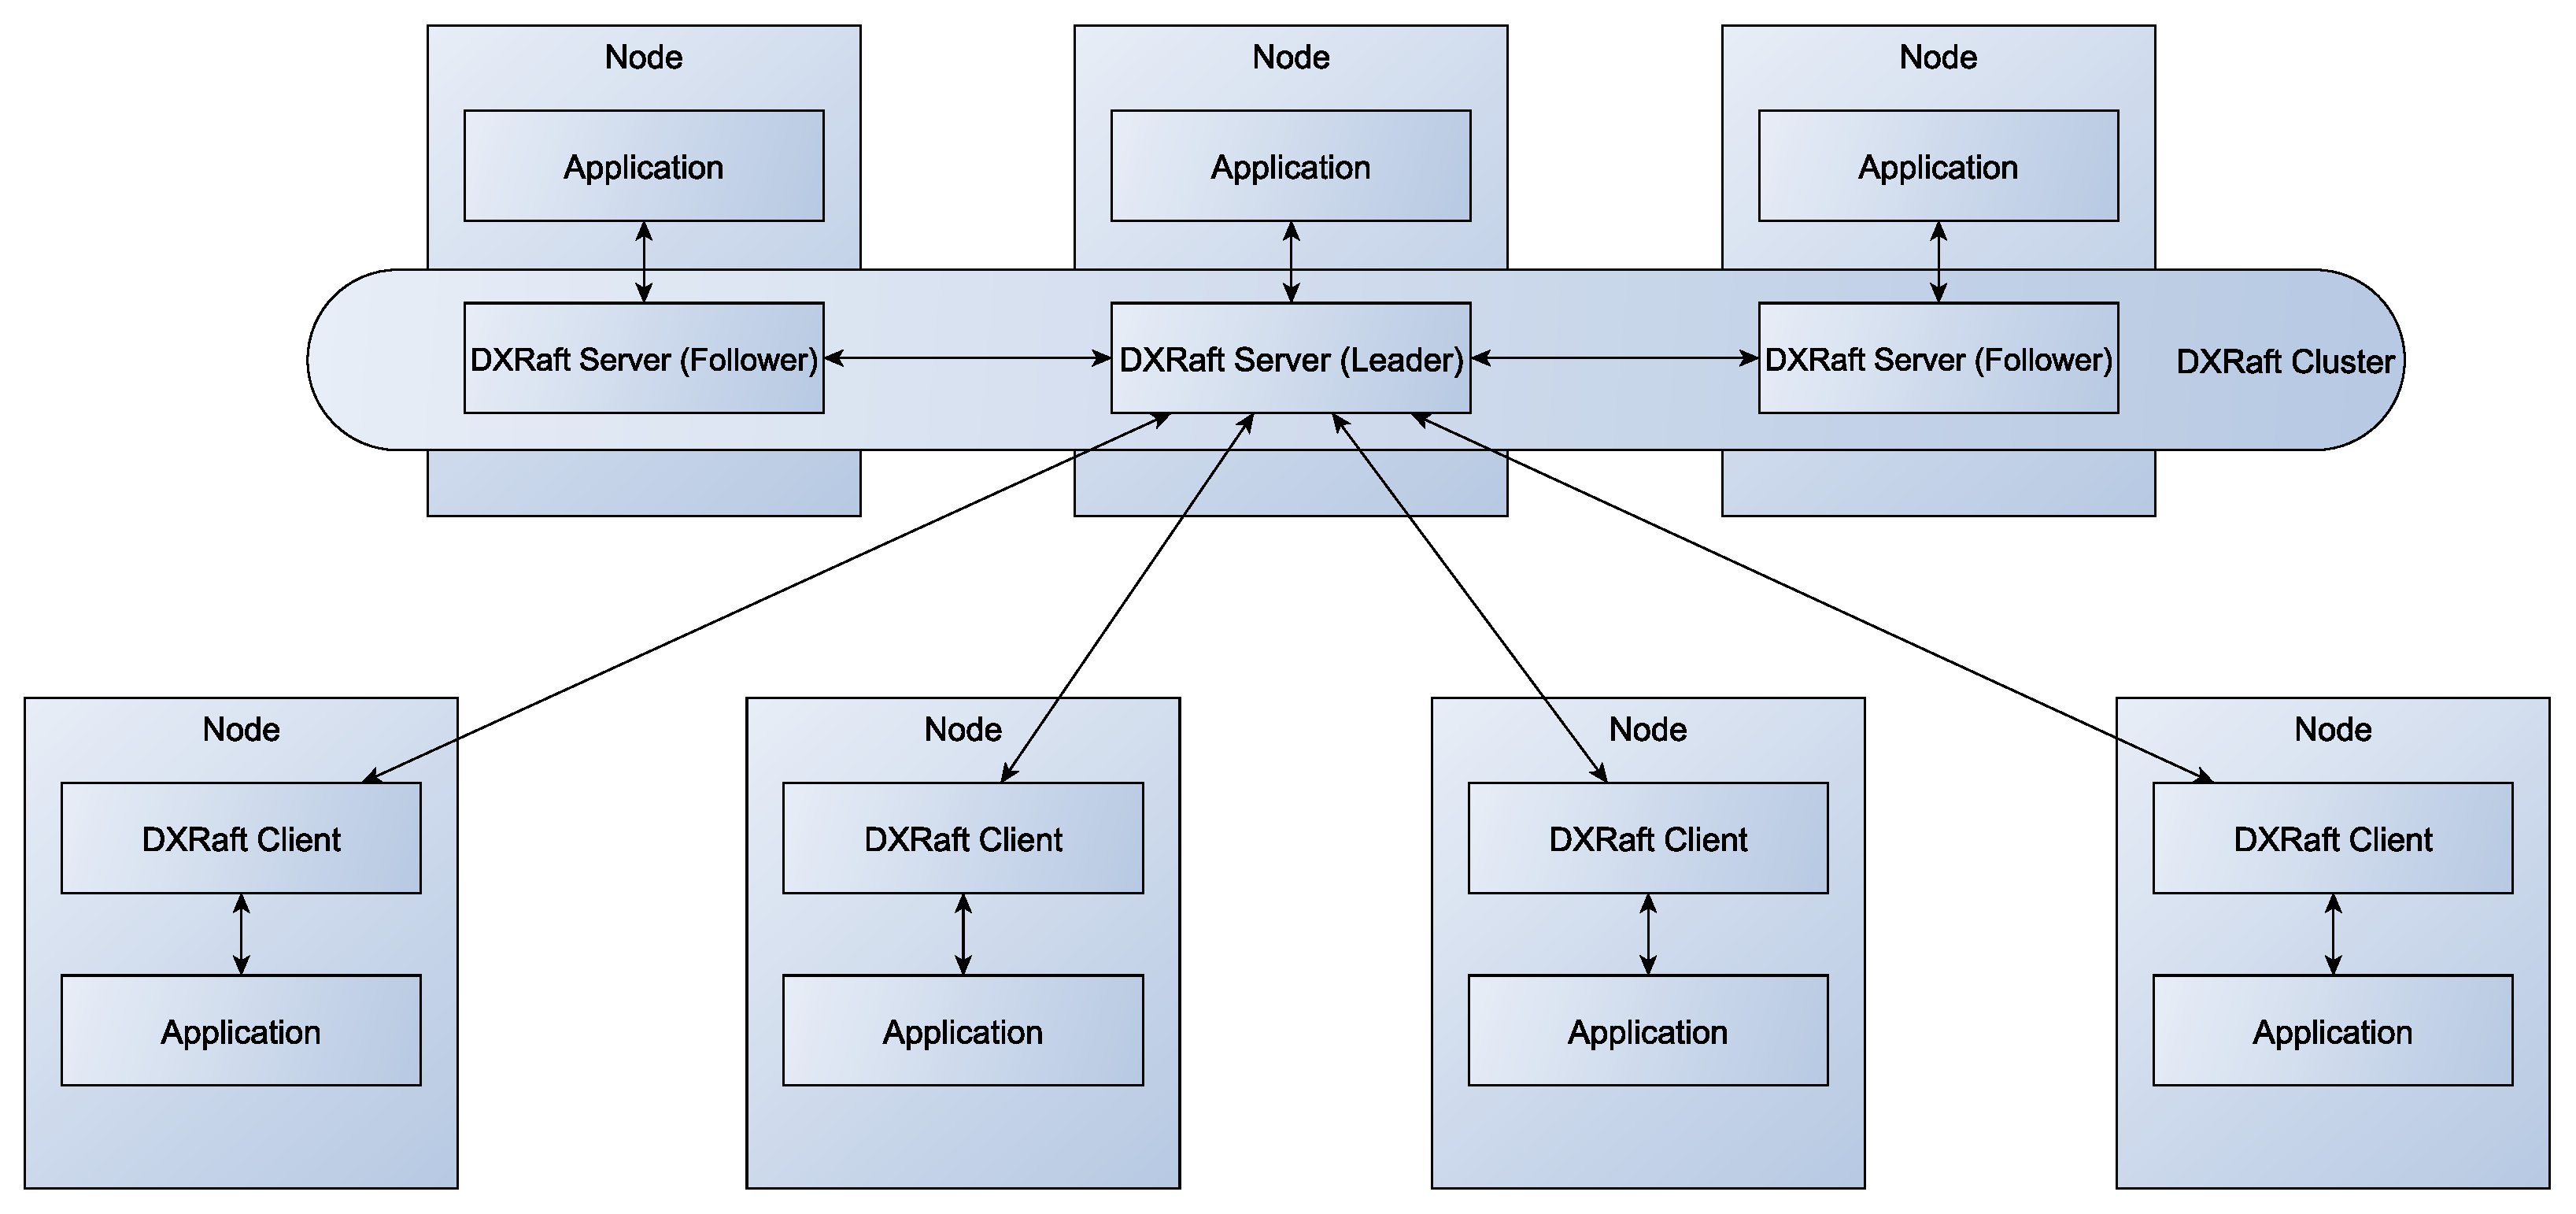
\includegraphics[width=\linewidth]{img/components.pdf}
	\caption{Beispiel für die Verwendung von DXRaft mit einer verteilten Anwendung.}
	\label{fig:components}
\end{figure}

Die Schnittstelle soll auf unterster Ebene eine Speicherung von Key-Value-Daten ermöglichen. Die Daten sollen mit einem String identifiziert werden und Daten von beliebigem Typ speichern. Außerdem sollen beliebige atomare Operationen auf den Daten ausgeführt werden können. Mit dieser Schnittstelle könnten dann weiter abstrahierte Funktionalitäten bzw. Klassen implementiert werden, wie z.B. eine \textit{DistributedAtomicInteger}-Klasse, die atomare Operationen auf einem im System gespeichertem Integer-Wert ausführt.

\section{Server}

Die Server-Instanzen bilden das Raft-Cluster und führen den Raft-Algorithmus durch. Dafür müssen sie die im Raft-Algorithmus definierten Daten speichern und zwischen den Status wechseln können. Ein Server kann mit der \textit{RaftServer}-Klasse erstellt und gestartet werden. Im Folgenden werden die Probleme erläutert, die bei der Implementierung aufgekommen sind, und die Konzepte erklärt, mit denen diese gelöst wurden.

\subsection{Messaging}
\label{messaging}

Da DXRaft ein verteiltes System ist, müssen die Instanzen über das Netzwerk kommunizieren. Um diese zu implementieren gibt es offensichtlich viele verschiedene Ansätze. Um bessere Möglichkeiten zur Optimierung zu bieten und die Implementierung leichtgewichtig zu halten, wird hier auf die Verwendung von fertigen Implementierungen wie DXNet  \cite{dxnet} oder MPI \cite{mpi} verzichtet. Da an die interne Kommunikation andere Anforderungen gestellt sind als an die externe Kommunikation mit Clients, sind diese in DXRaft getrennt und es wird jeweils ein eigener Socket geöffnet. Hier soll es zunächst um die Kommunikation zwischen den Server-Instanzen gehen. In \ref{client-messaging} wird dann die Kommunikation zwischen Client und Server genauer beschrieben.

Zunächst muss ein Transportschichtprotokoll festgelegt werden, mit dem die Kommunikation ablaufen soll. 
Der Raft-Algorithmus nutzt eine Nachrichtensemantik, das heißt die Server senden sich gegenseitig einzelne Nachrichten und keinen Strom von Daten. Außerdem wurde beim Entwurf des Algorithmus bereits ein unzuverlässiges Netzwerk berücksichtigt, welches verlorene Nachrichten erlaubt. Deshalb wird in DXRaft UDP genutzt. Das Messaging ist jedoch mithilfe von \textit{NetworkService}-Interfaces modular aufgebaut, sodass der Nachrichtenaustausch nachträglich auch anders implementiert werden könnte. Es könnte z.B. sinnvoll sein, TCP-Verbindungen zwischen den Raft-Servern aufzubauen, um die Verbindungen zu überwachen und schnell Ausfälle zu erkennen. Da in einem Raft-Cluster normalerweise eine eher kleine Anzahl an Servern teilnimmt, ist der Aufwand für das Verwalten der Verbindungen zu vernachlässigen.

Der UDP-Socket wird von einem Thread überwacht, der die Nachrichten deserialisiert und je nach Nachrichtentyp verarbeitet. Das sollte zunächst für die vorgesehenen Einsatzzwecke genügen. Falls die Performance später noch verbessert werden sollte, wäre es eventuell sinnvoll, die Verarbeitung von einem oder mehreren separaten Threads übernehmen zu lassen und/oder mehrere Threads pro Socket einzusetzen, die die Nachrichten deserialisieren. Damit könnte mehr Parallelität erreicht werden.

In Abbildung \ref{fig:server-messages} sind alle Nachrichten beschrieben, die zwischen den Servern ausgetauscht werden. Vote-Requests und -Responses werden von Candidates an Follower geschickt, Append-Entries-Requests und -Responses vom Leader an Follower geschickt.

\begin{figure}[h]
	\footnotesize
	\begin{tabular}{ | l | l | l | l |}	
		\hline
		\multirow{2}{*}{Name} & \multirow{2}{*}{Beschreibung} & \multicolumn{2}{|c|}{Inhalt}  \\ \cline{3-4}
		& & Name & Typ \\ \hline
		\multirow{6}{*}{Append-Entries-Request} & \multirow{6}{0.3\textwidth}{Leader sendet Einträge an die Follower, die diese an ihr Log anhängen sollen.} 
		& id & long \\
		& & term & int \\ 
		& &  prevLogIndex & int \\
		& &  prevLogTerm & int \\ 
		& & leaderCommitIndex &  int \\
		& & entries & List\textless{}LogEntry\textgreater \\ \hline
		\multirow{4}{*}{Append-Entries-Response} &  \multirow{4}{0.3\textwidth}{Antwort an den Leader, ob die Einträge erfolgreich angehängt wurden.} 
		& id & long\\
		& & term & int \\
		& & success & boolean \\
		& & commitIndex & int \\ \hline
		\multirow{3}{*}{Vote-Request} &  \multirow{3}{0.3\textwidth}{Candidate möchte Stimmen der Follower erhalten.} 
		& term & int \\
		& & lastLogIndex & int \\
		& & lastLogTerm & int \\ \hline
		\multirow{2}{*}{Vote-Response} &  \multirow{2}{0.3\textwidth}{Antwort an den Candidate, ob die Stimme gegeben wurde.} & term & int\\
		& & voteGranted & boolean \\ \hline
	\end{tabular}
	\caption{Nachrichtentypen bei der Kommunikation zwischen den Servern.}
	\label{fig:server-messages}
\end{figure}

Da UDP zum Senden von Anfragen genutzt wird, muss das erneute Senden auf der Anwendungsebene übernommen werden. Dafür überwacht der Leader für jeden Append-Entries- und Vote-Request an die Follower die Zeit bis zur Antwort. Falls er die Antwort nicht rechtzeitig erhält, sendet er die Anfrage erneut. Die Anfragen und Antworten werden mit einer aufsteigenden Zahl identifiziert, die der Leader beim Senden vergibt. Um die Korrektheit zu garantieren, sendet der Leader an jeden Follower höchstens eine Anfrage gleichzeitig. Mit einem Append-Entries-Request können jedoch mehrere Log-Einträge versendet werden, falls während eines Anfrage-Antwort-Zyklus bereits mehrere Einträge an das Log angehangen wurden. Dadurch wird eine Batch-Verarbeitung erreicht, bedingt durch die Einschränkung, dass nur ein Append-Entries-Request gleichzeitig gesendet werden kann. Die Batches haben eine dynamische Größe, werden jedoch durch einen Konfigurationsparameter in der Größe beschränkt. Außerdem wird die Größe durch die maximale Größe eines UDP-Paketes beschränkt, die nicht überschritten werden darf.\\
Auch hier könnte man die Perfomance möglicherweise erhöhen, indem mehrere parallele Anfragen an die Follower erlaubt werden. Dann müsste jedoch sichergestellt werden, dass die Anfragen vom Follower in der richtigen Reihenfolge verarbeitet werden (z.B. durch Verwendung von TCP) und eine Flusskontrolle implementiert werden, die die Anzahl der parallel gesendeten Anfrage vorgibt.

\subsection{Bootstrapping}

\begin{figure}[p]
	\centering
	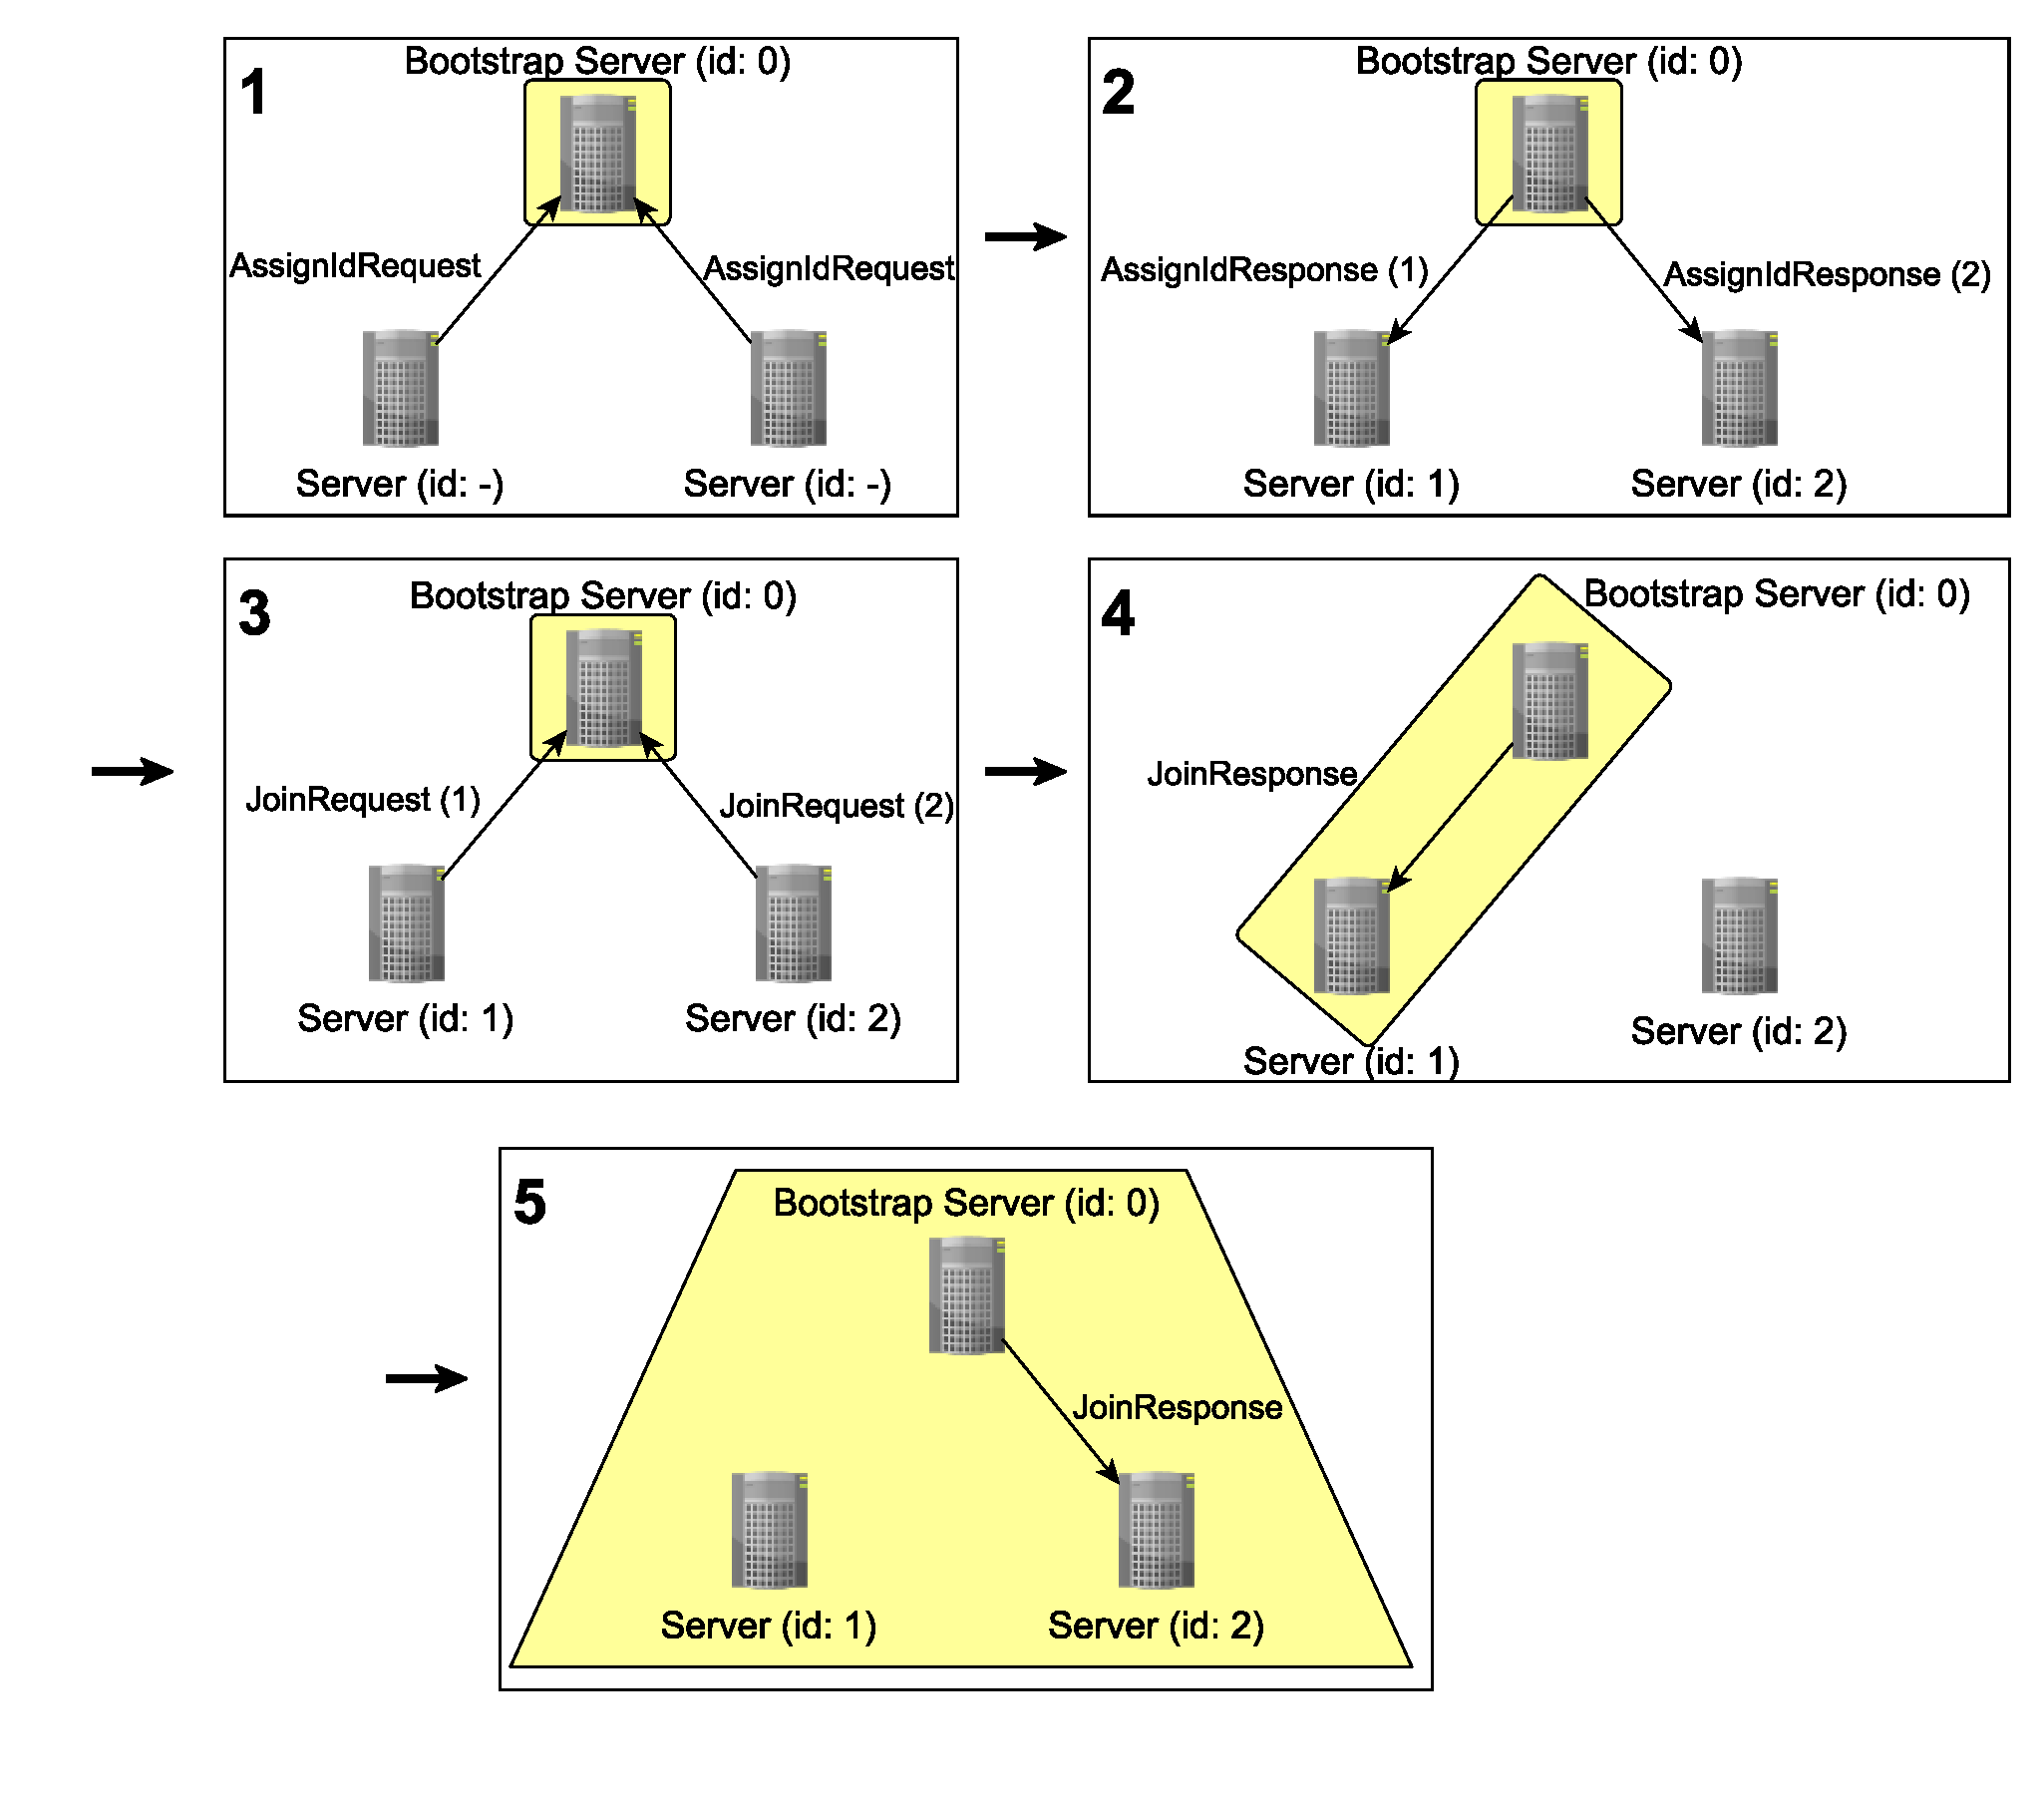
\includegraphics[width=\linewidth]{img/bootstrap.pdf}
	\caption{Dynamischer Bootstrapping-Prozess mit drei Servern. Alle Nachrichten werden über IP-Multicast gesendet. Der gelbe Bereich gibt an, welche Server gerade Teil des Clusters sind.}
	\label{fig:bootstrap}
\end{figure}

Um den Raft-Algorithmus durchzuführen und insbesondere festzustellen, wann eine Mehrheit der Server eine Anfrage akzeptiert hat, muss jeder teilnehmender Server alle anderen teilnehmenden Server kennen. Diese Information muss den Servern beim Bootstrapping bekannt gemacht werden. Eine einfache Möglichkeit ist, jeder Server-Instanz alle teilnehmenden Server mit ihren Adressen \textbf{statisch} beim Start per Konfigurationsdatei zu übergeben. Dies wird so auch in einigen Systemen, wie z.B. Zookeeper, so gelöst und ist auch in DXRaft eine Möglichkeit, die Server zu starten. 

Dies ist jedoch nicht sehr komfortabel, da alle teilnehmenden Server mit ihren Adressen manuell oder mit einem eigens dafür geschriebenem Skript eingetragen werden müssen. Deshalb gibt es in DXRaft die Möglichkeit, dass die Server sich automatisch finden und den Cluster \textbf{dynamisch} aufbauen. Abbildung \ref{fig:bootstrap} zeigt den Ablauf des dynamischen Bootstrappings mit 3 Servern. In Abbildung \ref{fig:bootstrap-messages} sind zudem die Nachrichten beschrieben, die dabei ausgetauscht werden. Zunächst muss eine Server-Instanz als Bootstrap-Instanz gewählt werden, die damit beginnt, ein Cluster aufzubauen. Dieser Server fügt sich selbst in die Liste der teilnehmenden Server ein und erstellt dafür einen Log-Eintrag, der über den normalen Raft-Mechanismus später auf alle teilnehmenden Server repliziert wird. Dann öffnet er einen Multicast-Socket und wartet, bis er darüber Join-Requests von anderen Servern erhält. Ein Join-Request beinhaltet die Adresse des Servers, der dem Cluster beitreten möchte, sodass das Beitreten über den Beitrittsmechanismus (beschrieben in \ref{config-change}) gestartet werden kann. Da jeder beitretende Server dadurch auch das gesamte Log übergeben bekommt, bekommt er auch die Adressen aller Server mitgeteilt, die bereits vor ihm dem Cluster beigetreten sind. Falls die Bootstrap-Instanz, die initial der Leader ist, abstürzt, nachdem bereits ein oder mehrere Server dem Cluster beigetreten sind, wird der nächste Leader zur Bootstrap-Instanz. So kann der Boot-Vorgang auch weiterhin fortgeführt werden.

\begin{figure}[h]
	\footnotesize
	\begin{tabular}{ | l | l | l | l |}	
		\hline
		\multirow{2}{*}{Name} & \multirow{2}{*}{Beschreibung} & \multicolumn{2}{|c|}{Inhalt}  \\ \cline{3-4}
		& & Name & Typ \\ \hline
		Assign-Id-Request & Ein Server möchte eine \textit{id} erhalten. 
		& requestId & UUID \\ \hline
		\multirow{2}{*}{Assign-Id-Response} &  \multirow{2}{0.35\textwidth}{Antwort vom Leader an den Server mit einer \textit{id}.} 
		& requestId & UUID \\
		& & id & int \\ \hline
		\multirow{2}{*}{Join-Request} &  \multirow{2}{0.35\textwidth}{Ein Server mit einer \textit{id} möchte dem Cluster beitreten.} 
		& requestId & UUID \\
		& & address & RaftAddress (id, ip und port)\\ \hline
		\multirow{2}{*}{Join-Response} &  \multirow{2}{0.35\textwidth}{Antwort vom Leader an den Server, ob der Beitritt erfolgreich war.} & requestId & UUID\\
		& & success & boolean \\ \hline
	\end{tabular}
	\caption{Nachrichtentypen beim dynamischen Bootstrapping. Die Nachrichten werden mit einer UUID (\textit{requestId}) identifiziert, da sie auch identifiziert werden müssen, wenn mehrere Server gleichzeitig Nachrichten über Multicast senden.}
	\label{fig:bootstrap-messages}
\end{figure}

Außerdem müssen die Server eindeutig identifiziert werden, damit der Raft-Algorithmus korrekt funktioniert. Deshalb hat jede Server-Instanz in DXRaft einen Integer-Identifier \textit{id}. Bei statischer Konfiguration muss die \textit{id} in der Konfigurationsdatei mit den Adressen der Server übergeben werden. Bei dynamischer Konfiguration werden die \textit{ids} ebenfalls dynamisch vergeben. Dazu wird wieder der Raft-Mechanismus selber verwendet: Die Bootstrap-Instanz gibt sich selbst die \textit{id} 0 und erstellt einen \textit{Atomic Integer}-Eintrag für die Vergabe der \textit{ids}. Die Server, die dem Cluster beitreten wollen, müssen sich dann zunächst nach dem Start eine \textit{id} besorgen. Dafür senden sie über IP-Multicast einen Assign-Id-Request. Wenn die Bootstrap-Instanz (oder der aktuelle Leader) die Anfrage bekommt, führt diese ein atomares \textit{GetAndIncrement} auf dem \textit{Atomic-Integer}-Eintrag durch und sendet die erhaltene \textit{id} zurück. Dann kann der Server den Beitritt zum Cluster wie bereits beschrieben starten.

Wie bei Client-Anfragen muss auch bei Join-Requests und Assign-Id-Request über Multicast sichergestellt werden, dass diese nicht doppelt durchgeführt werden, falls der Sender keine Antwort auf seine Anfrage bekommt und dieselbe Anfrage erneut sendet. Dazu bekommt jede Anfrage eine UUID \cite{uuid}. Eine dedizierte Session wird bei der Bootstrap-Instanz verwendet, um die Multicast-Anfrage und die Ergebnisse zu speichern, sodass diese nicht doppelt ausgeführt werden können (siehe \ref{sessions} für die Erklärung des Session-Mechanismus bei (Client-)Anfragen). Diese dedizierte Session ist momentan unbegrenzt groß, da es normalerweise nicht allzu viele Multicast-Anfragen geben sollte, sodass sie den Speicher nicht zu sehr belastet. Die UUID wird auch mit der Antwort gesendet, damit der anfragende Server die Antwort identifizieren kann.

Die statische Konfiguration ist etwas sicherer, falls einer oder mehrere  Server bereits während des Boot-Vorgangs abstürzen sollten. Da alle Server bereits alle Server kennen, können keine Anfragen bearbeitet werden, wenn keine Mehrheit erreicht werden kann. Bei dynamischer Konfiguration ist bei Anfragen während des Boot-Vorgangs nicht sichergestellt, dass bereits alle Server dem Cluster beigetreten sind. Falls dies nicht der Fall ist, dann ist die Fehlertoleranz eventuell schlechter als erwartet, da weniger Server am Cluster teilnehmen und die Mehrheit anders berechnet wird. Dies könnte gelöst werden, indem dem Cluster eine Zahl übergeben wird, die angibt, ab welcher Anzahl an beigetretenen Servern Anfragen beantwortet werden können. Dann kann jedoch ein einziger Server, der ausfällt, den Boot-Vorgang fehlschlagen lassen.

Aus diesen Gründen kann man je nach Anforderungen per Parameter das Bootstrapping statisch oder dynamisch durchführen.

\subsection{Persistenz}

Im Raft-Algorithmus ist es vorgesehen, dass sich Server nach einem Absturz wieder erholen können und nach einem \textit{Recover}-Vorgang wieder am Cluster teilnehmen können, ohne das korrekte Arbeiten des Algorithmus zu stören. Dazu müssen wichtige Daten, wie z.B. der \textit{current term} oder das Log, synchron auf der Festplatte gesichert werden, sodass diese bei einem möglichen Absturz nicht verloren gehen. Dies ist in DXRaft noch nicht implementiert und die Wiederherstellung wird momentan dem Systemadminstrator überlassen (z.B. durch das Entfernen und erneute Hinzufügen des Servers zum Cluster über den Beitrittsmechanismus).

Dennoch muss das Log bereits ohne die Möglichkeit der Wiederherstellung persistiert werden: Da bei jeder Anfrage ein Eintrag in das Log geschrieben wird, wird das Log schnell sehr groß. Falls das Log nur im Speicher gehalten wird, belastet es auch sehr stark den Garbage Collector und die Garbage-Collector-Pausen werden sehr lang (\textgreater 500 ms), wodurch die Timeouts nicht mehr richtig funktionieren und es zu unnötigen Leaderwechseln kommt. Außerdem kann das Log dann auch schnell den gesamten Speicher ausfüllen. Deswegen ist es nötig, das Log auf der Festplatte zu persistieren. Da Festplattenzugriffe sehr viel mehr Zeit benötigen als Speicherzugriffe, muss das Log möglichst effizient gespeichert werden und die Zugriffe minimiert werden, damit die Performance nicht zu sehr leidet.

Das Log muss durch das Replizieren auf die anderen Server gelesen werden können. Insbesondere wird auf die neuesten Einträge häufig zugegriffen, während es unwahrscheinlich ist, dass auf ältere Einträge zugegriffen werden muss. Dennoch muss das Log theoretisch bis zum Anfang gelesen werden können, da Follower beliebig viele Nachrichten des Leaders nicht bekommen und dadurch beliebig viele Einträge nicht mitbekommen könnten. Um diese dann auf die betroffenen Follower zu replizieren, sobald diese wieder Nachrichten erhalten, müssen alte Einträge gelesen werden. Außerdem muss bei einem Beitritt eines neuen Servers das gesamte Log auf den neuen Server übertragen werden.

Weiterhin müssen auch Einträge am Ende des Logs gelöscht werden können. Dies kann bei Leaderwechseln nötig werden, wenn der Leader die Logs der Follower seinem Log angleicht und es Einträge gibt, die im Log des Followers vorhanden sind aber nicht im Log des Leaders.

\begin{figure}[h]
	\centering
	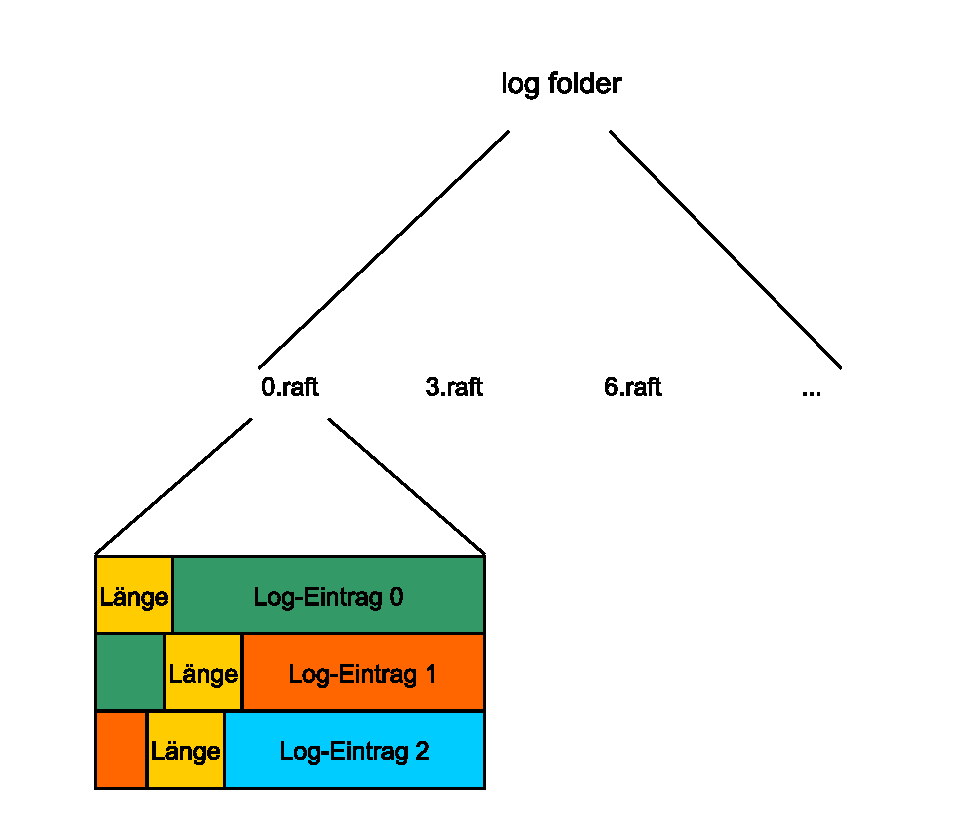
\includegraphics[width=300px]{img/log-files.pdf}
	\caption{Persistierung des Logs auf Festplatte. Hier hat jede Log-Datei maximal drei Einträge. Der Name der Datei (z.B. \textit{3.raft}) gibt den Log-Index des ersten Eintrags, der in der Datei gespeichert ist, an. In der Datei wird für jeden Eintrag die Länge des Eintrags vor den Eintrag geschrieben, damit die Datei nach einem speziellen Eintrag durchsucht werden kann.}
	\label{fig:log-files}
\end{figure}

Die Einträge des Logs sind beliebig groß, weswegen die Länge der Einträge in der Log-Datei mitgespeichert werden muss, um die Einträge wiederzufinden. Dadurch kann nicht direkt mit einem Index auf den entsprechenden Eintrag zugegriffen werden. Die naive Lösung ist, die Länge des Eintrags immer vor dem Eintrag zu speichern und beim Lesen eines Eintrags die Log-Datei von Beginn an zu durchsuchen, indem immer die Länge des nächsten Eintrags gelesen wird und diese Anzahl an Bytes übersprungen wird, bis der gesuchte Eintrag gefunden wurde. Dies ist aber offensichtlich keine gute Lösung, da das Suchen eines Eintrags dadurch linear mit der Länge des Logs steigt.

Eine weitere Möglichkeit wäre es, eine zusätzliche Datei anzulegen, die zu jedem Index die Adresse des Eintrags in der Log-Datei speichert. Dann könnte der Zugriff in konstanter Zeit erfolgen, falls man davon ausgeht, dass die Indexdatei in konstanter Zeit gelesen werden kann. Dann müsste jedoch beim Anhängen eines Log-Eintrags mindestens zwei Mal auf die Festplatte geschrieben werden, einmal um den Eintrag in die Log Datei zu schreiben und einmal um die Adresse in die Indexdatei zu schreiben. Da die Zugriffe wegen der Fehlertoleranz immer synchron geschehen müssen, erhöhen sie die Latenz von Client-Anfragen deutlich. Deshalb wäre es gut, wenn das Anhängen auf einen Schreib-Zugriff reduziert werden könnte.

Dafür nutzt DXRaft die bereits vorhandene Baumstruktur des Dateisystems. Abbildung \ref{fig:log-files} veranschaulicht diese Lösung. Das Log wird in mehrere Dateien aufgeteilt, die eine maximale Größe haben. Sobald das Anhängen eines Log-Eintrags die maximale Größe der Log-Datei überschreiten würde, wird eine neue Log-Datei angelegt und der Eintrag in diese neue Datei geschrieben. Der Index des ersten Eintrags, der in der dieser Datei gespeichert ist, wird im Namen der Datei gespeichert. Beim Lesen eines Eintrags kann dann mithilfe des Verzeichnisses die Datei ermittelt werden, in der dieser Eintrag gespeichert ist. Die Datei kann dann wie in der naiven Lösung nach dem Eintrag durchsucht werden. Dadurch ist das Lesen durch die maximale Größe einer Log-Datei beschränkt und das Schreiben benötigt normalerweise nur einen Schreibzugriff. Dazu kommt nur das Anlegen einer neuen Datei, falls eine Log-Datei zu groß geworden ist. Um die Schreib- und Lesezugriffe auf die Festplatte weiter zu minimieren, wird außerdem gepuffert gelesen und geschrieben (mit den \textit{BufferedReader}- und \textit{BufferedWriter}-Klassen aus dem \textit{java.io}-Package).
		
Dies könnte durch Batch-Verarbeitung von Anfragen noch weiter reduziert werden, wobei dann nur ein Schreibzugriff für das Anhängen mehrerer Einträge nötig wäre. Da dies jedoch nicht ganz einfach zu implementieren ist und die Performance auch ohne Batch-Verarbeitung bereits ausreichend ist, wurde dies im Rahmen dieser Arbeit noch nicht implementiert.

Da die neuesten Einträge des Logs häufig gelesen werden müssen, werden diese außerdem noch in einem Cache gehalten. Der Cache hält die letzten \textit{n} Einträge im Speicher und es wird der älteste entfernt, falls der Cache voll ist und ein neuer Eintrag an das Log angehängt wird. Da im Normalbetrieb nur auf die neuesten Einträge zugegriffen wird, kann durch einen ausreichen großen Cache erreicht werden, dass im Normalbetrieb kein Lesezugriff auf die Festplatte erfolgt.

Da auch auf der Festplatte nicht unendlich Speicherplatz vorhanden ist, kann das Log auch diesen Platz irgendwann aufbrauchen. Damit das System dann weiterhin funktioniert, muss eine Kompaktierung des Logs implementiert werden. Dazu haben die Raft-Autoren ebenfalls einen Mechanismus entwickelt, der jedoch in DXRaft noch nicht implementiert wurde.

\subsection{Änderungen der Clusterkonfiguration}
\label{config-change}

\begin{figure}[p]
	\centering
	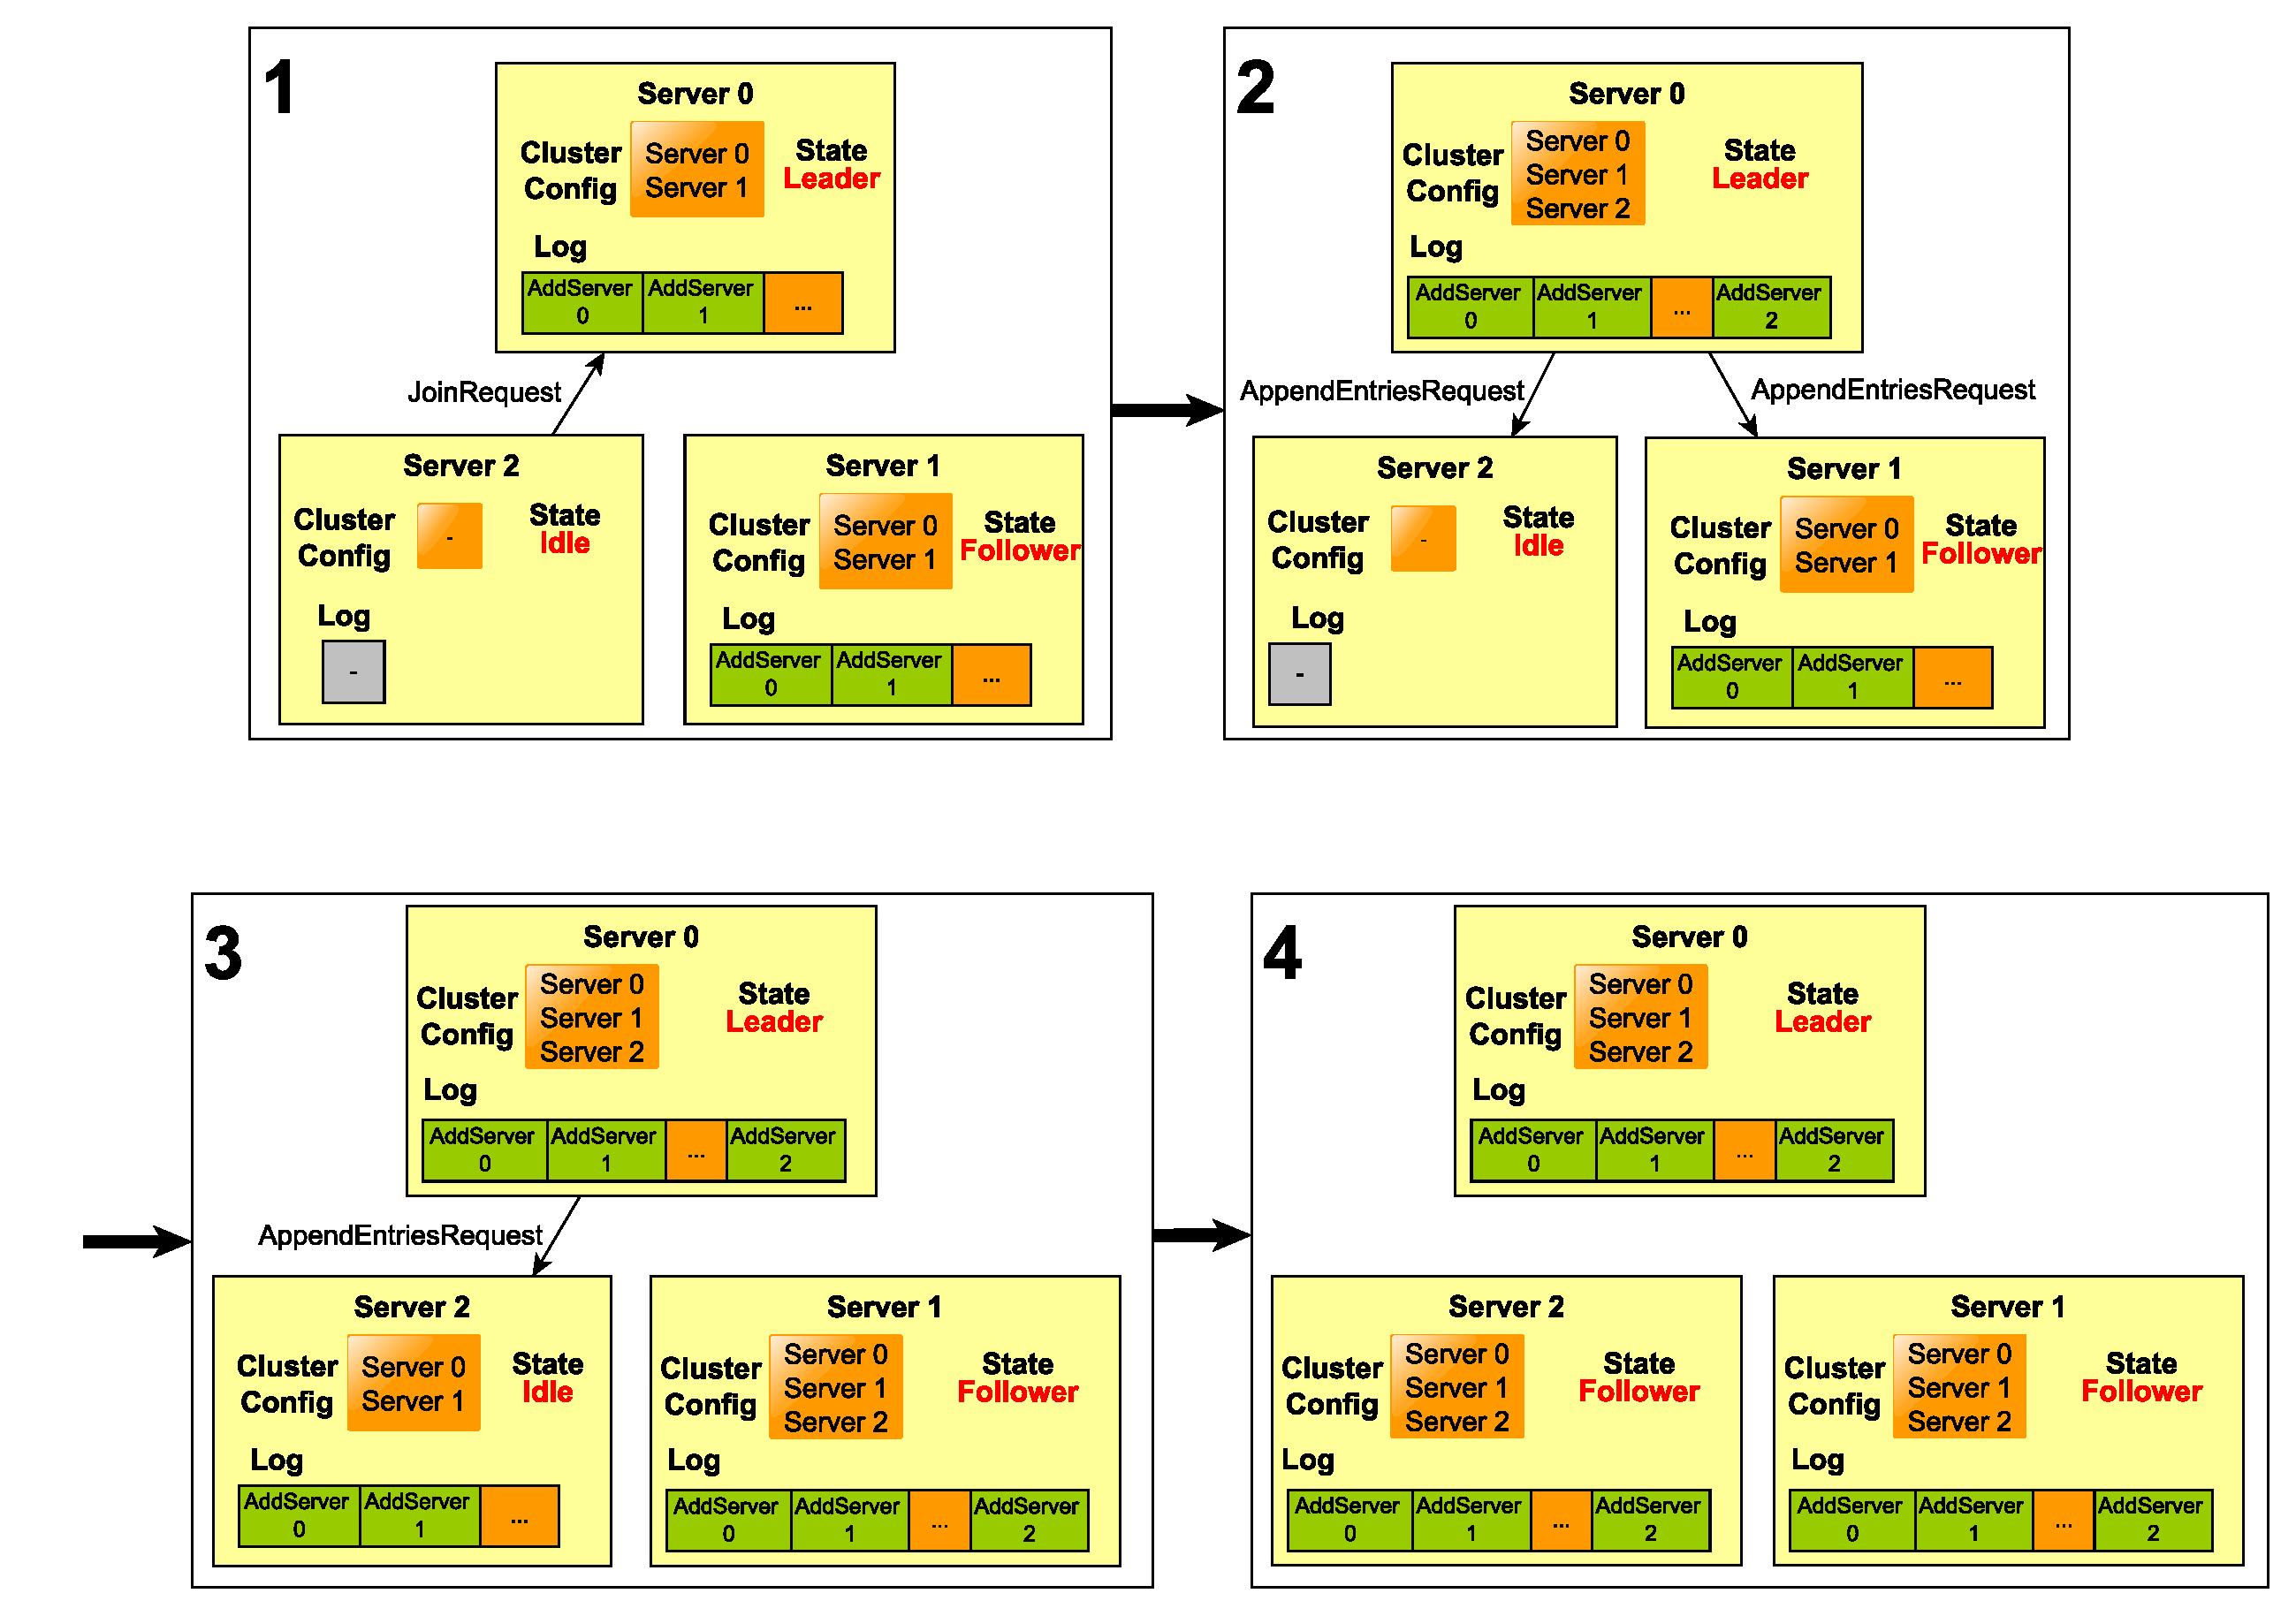
\includegraphics[width=\linewidth]{img/config-change.pdf}
	\caption{Ablauf einer Änderung der Cluster-Konfiguration. Server 2 möchte dem Cluster beitreten, das momentan aus Server 0 und Server 1 besteht. Er startet im Idle-Status und sendet einen Join-Request an den Leader. Dann bekommt er das aktuelle Log über den Raft-Replikationsmechanismus mitgeteilt. Darin enthalten sind frühere Änderungen an der Cluster-Konfiguration. Daher kann er die aktuelle Cluster-Konfiguration erstellen. Sobald er den Eintrag erhält, in dem er selbst zum Cluster hinzugefügt wird, nimmt er aktiv am Cluster teil und wird zum Follower.}
	\label{fig:config-change}
\end{figure}

Im laufenden Betrieb kann es vorkommen, dass man die Menge der am DXRaft-Cluster teilnehmenden Server ändern möchte, z.B. möchte man einen ausgefallenen Server durch einen neuen ersetzen. Währenddessen sollte das Cluster nach Möglichkeit weiterhin funktionieren und Anfragen beantworten. Wenn in einer Konfigurationsänderung mehrere Server dem Cluster beitreten oder aus dem Cluster austreten, kann es passieren, dass während der Konfigurationsänderung zwei Mehrheiten für Leader entstehen, da die Konfigurationsänderung nicht allen Servern im Cluster gleichzeitig bekannt gemacht werden kann. Daraus könnte dann resultieren, dass zwei Leader in einem Term existieren. Das würde die Sicherheitsbedingung von Raft verletzten und zu Inkonsistenzen führen.

Die von den Raft-Entwicklern vorgeschlagene Lösung ist, nur einem Server gleichzeitig zu erlauben, dem Cluster beizutreten oder aus dem Cluster auszutreten. Dabei können keine zwei Mehrheiten gleichzeitig entstehen. Wenn mehrere Server dem Cluster beitreten wollen, muss das Beitreten sequentiell ablaufen. Diesen Mechanismus nutzt auch DXRaft.

Abbildung \ref{fig:config-change} zeigt den Ablauf einer Änderung an der Cluster-Konfiguration. Ein Beitritt eines Servers kann entweder von dem Server selbst oder von einem Client initiiert werden. Wenn der Server selbst den Beitritt initiiert, sendet er einen Join-Server-Request über IP-Multicast. Falls Broadcasting in der Konfigurationsdatei deaktiviert ist, startet der Server im Idle-Modus und wartet auf Nachrichten des Leaders. Dann muss ein Client den Beitritt initiieren, indem er einen Add-Server-Request mit der Adresse des beitretenden Servers sendet. Unabhängig davon, wer den Beitritt initiiert, läuft der Beitritt gleich ab: Der Leader prüft zunächst, ob bereits eine Konfigurationsänderung läuft. Falls dies der Fall ist, wird die Anfrage in eine Warteschlange eingefügt. Sobald die laufende Konfigurationsänderung abgeschlossen ist, wird die nächste Änderung gestartet. Auch für Konfigurationsänderungs-Anfragen wird das Log genutzt, um diese allen Servern konsistent bekannt zu machen. Es wird ein Log-Eintrag für jede Konfigurationsänderung angelegt und sobald dieser Eintrag auf einer Mehrheit der Server repliziert wurde, ist die Änderung abgeschlossen und kann beantwortet werden. Die Server fügen den beitretenden Server in ihre Liste der bekannten Server ein, sobald sie den entsprechenden Eintrag an ihr Log anhängen. Der neue Server bekommt über den normalen Replikations-Mechanismus mit Append-Entries-Requests das gesamte Log geschickt, sobald er dem Leader bekannt ist.

Ein Austreten eines Servers muss von einem Client initiiert werden. Der Austritt läuft analog zum Beitritt ab. Sobald der Austritt vom Leader bestätigt wurde, kann der Server abgeschaltet werden. Ein automatisches Ausschließen von nicht antwortenden Servern aus dem Cluster ist problematisch, da nicht festgestellt werden kann, ob der Server abgestürzt ist oder nur die Nachrichten verloren gehen. Dadurch könnte es passieren, dass ein Server ausgeschlossen wird, obwohl er noch aktiv ist. Dieser könnte dann die Arbeit des restlichen Clusters beeinträchtigen, z.B. indem er periodisch eine Leader-Wahl initiiert. Außerdem würde durch ein automatisches Verkleinern des Clusters der Replikationsgrad verringert werden, wodurch das System an Sicherheit verliert.

Zur Optimierung des Beitritts könnte noch ein zusätzlicher \glqq Recovery \grqq-Mechanismus implementiert werden, durch den das Log des neuen Servers auf den Stand des Logs des Leaders gebracht wird bevor der Beitritt gestartet wird. Da dabei das gesamte Log an den neuen Server geschickt werden muss, wäre es sinnvoll das Lesen und Senden vieler Log-Einträge zu optimieren, z.B. durch paralleles Lesen aus der Log-Datei. Diese Optimierungen wären bei dem normalen Replikations-Mechanismus nicht sinvoll, da dabei die Server meist nicht so viele Einträge erhalten müssen und die Einträge auch meistens aus dem Cache gelesen werden können.

\subsection{Timer}

Die Server müssen aus unterschiedlichen Gründen die Zeit im Auge behalten und einen Timeout auslösen, falls ein Ereignis zu lange auf sich warten lässt:

\begin{itemize}
	\item Leader müssen periodisch einen Heartbeat senden, falls das System gerade keine Anfragen bearbeitet und das System gerade keine Anfragen bearbeitet.
	\item Candidates müssen eine neue Wahl starten, wenn die Wahl in einer Zeitspanne keinen Sieger hervorgebracht hat.
	\item Follower müssen einen eine Wahl starten, wenn sie zu lange keine Nachricht vom Leader erhalten haben.
\end{itemize}

Diese Funktionalität wird durch die \textit{RaftTimer}-Klasse bereitgestellt. Diese verwendet intern einen \textit{ScheduledExecutorService}, der, wenn aktiviert, auslöst, sobald eine vorher übergebene Zeit abgelaufen ist. Dann wird die \textit{processTimeout()}-Methode eines vorher übergebenen \textit{TimeoutHandlers} aufgerufen. 

Damit die Server im Cluster möglichst nicht zur gleichen Zeit einen Timeout auslösen, sollte die Zeitspanne randomisiert werden. Dafür kann der \textit{RaftTimer}-Klasse ein fixe Zeit \textit{f} und zusätzliche randomisierte Zeit \textit{r} übergeben werden. Der Timer löst dann frühestens aus, nachdem \textit{f} abgelaufen ist, und spätestens, nachdem \textit{f+r} abgelaufen ist.

Außerdem wird der Timer auch für die Überwachung von Append-Entries- und Vote-Requests genutzt. Diese müssen nach dem Ablauf des Timers erneut gesendet werden, falls der Leader in dieser Zeit keine Antwort erhalten hat (siehe \ref{messaging}).

\section{Client}

Der Client bildet die Schnittstelle von DXRaft zur Anwendung. Er wird als Library in die Anwendung eingebunden und leitete die Anfragen von der Anwendung an das DXRaft-Cluster weiter. Standardmäßig werden die DXRaft-Server automatisch über Multicast gefunden. Falls dies nicht möglich, muss dem Client eine Liste der Server mit Adressen übergeben werden. Bei der Implementierung des Clients ist es vor allem wichtig, dass Fehler, wie z.B. das Ausbleiben einer Antwort von einem Server, korrekt behandelt wird. In \ref{sessions} wird beschrieben, wie es erreicht werden kann, dass die Anfragen immer genau ein mal ausgeführt werden. In \ref{api} wird dann die API genau beschrieben.

\subsection{Sessions}
\label{sessions}

Wenn der Client keine Antwort auf seine Anfrage bekommt, dann kann er nicht feststellen, ob die Anfrage erfolgreich durchgeführt wurde oder nicht. Wenn er dann sofort aufgeben würde, wäre das System nicht fehlertolerant. Deswegen sendet er die gleiche Anfrage erneut, um dem Server zu signalisieren, dass er keine Antwort erhalten hat. Dies könnte jedoch ohne weitere Maßnahmen dazu führen, dass die Anfrage mehrfach bearbeitet wird. Das wäre für den Nutzer jedoch unerwartet und würde bedeuten, dass das System nicht korrekt arbeitet. Um die mehrfache Bearbeitung einer Anfrage zu verhindern, müssen die Anfragen mit dem Ergebnis serverseitig gespeichert werden, sodass der Server feststellen kann, ob er die Anfrage bereits einmal erhalten hat und das Ergebnis zurücksenden kann, falls diese bereits durchgeführt wurde.

Leider können nicht alle Anfragen mit dem Ergebnis gespeichert werden, da dann das gesamte Log im Speicher gehalten werden müsste und auch bei jeder Anfrage komplett durchsucht werden müsste. Um diese Problematik zu lösen, werden die Daten in Sessions gespeichert, die eine begrenzte Anzahl Anfragen mit dem Ergebnis speichern. Jeder Client sendet dafür einen Create-Session-Request an das Cluster, bevor er irgendeine andere Anfrage stellt. Er bekommt dann die Session-Id der erstellten Session zurück. Jede Anfragen bekommt dann vom Client die Session-Id, die die Session der Anfrage identifiziert, und eine aufsteigenen Integer-Id, die die Anfrage in der Session identifiziert, zugewiesen. Dadurch ist jede Anfrage eindeutig identifiziert und kann wiedergefunden werden.

Wenn der Client so viele Anfragen gesendet hat, dass seine Session voll ist, werden seine Anfragen nicht mehr bearbeitet und der Server sendet einen \textit{SESSION\textunderscore FULL}-Error zurück. Dann muss die Session geleert werden. Dazu muss der Client zunächst sichergehen, dass er zu allen ausstehenden Anfragen eine Antwort erhalten hat. Dann kann er einen Purge-Session-Request senden, mit dem die Session geleert wird. Sobald dies erfolgreich geschehen ist, kann er weitere Anfragen stellen.

Da nicht unendlich viele Sessions im Speicher gehalten werden, müssens Sessions irgendwann auslaufen. Dies geschieht in DXRaft sobald eine bestimmte Zahl an Sessions erreicht ist. Dann wird die älteste Session invalidiert. Falls der Client der Session noch aktiv ist und eine weitere Anfrage sendet, wird ein \textit{SESSION\textunderscore EXPIRED}-Error gesendet. Es könnte dann Folgendes passiert sein: Die Anfrage wurde ausgeführt, die Antwort ist jedoch verloren gegangen. Bevor der Client die Anfrage erneut sendet, erstellt ein anderer Client eine Session. Da der Session-Speicher voll ist, muss die Session des ersten Clients gelöscht werden. Sobald dieser Client die vorherige Anfrage erneut sendet, bekommt er einen \textit{SESSION\textunderscore EXPIRED}-Error zurück. Die Anfrage wurde jedoch ausgeführt. Der Client kann dann also nicht mehr feststellen, ob seine Anfrage ausgeführt worden ist oder nicht. Deshalb wirft der Client in diesem Fall eine \textit{SessionExpiredException}. Es wird also dem Nutzer überlassen, wie dieser Fall behandelt werden soll. 

Durch die Anpassung der maximalen Anzahl an Sessions an die Anforderungen sollten sich ausgelaufene Sessions von aktiven Clients vermeiden lassen. Es könnten auch andere Verdrängungsstrategien für den Session-Speicher implementieren wie z.B. Least-Recently-Used or zeitbasierte Invalidierung. Bei zeitbasierter Invalidierung müsste jedoch sichergestellt werden, dass sich das gesamte DXRaft-Cluster auf die Zeit einigt, ab der die entsprechende Session invalidiert wird.

Damit die Sessions dem gesamten DXRaft-Cluster bekannt sind und bei einem Leaderwechsel weiter funktionieren, werden die \textit{CreateSession}- und \textit{PurgeSession}-Requests genau so behandelt wie andere Anfragen, das heißt sie werden mit dem Raft-Mechanismus repliziert und erst ausgeführt, wenn sie auf eine Mehrheit der Server repliziert wurden. Dadurch werden die Sessions auf jedem Server erstellt und die Server sind sich einig, wann eine Session geleert oder gelöscht wird.

\subsection{Messaging}
\label{client-messaging}

Auch für die Kommunikation zwischen Clients und Server wird in DXRaft UDP genutzt. Serverseitig übernimmt wie bei der Kommunikation zwischen den Servern ein Thread die Annahme der Nachrichten über den UDP-Socket und die Verarbeitung der Nachricht. Auch hier könnte TCP verwendet werden, jedoch könnte dies bei vielen Clients zu Performanceproblemen führen, da dann sehr viele Verbindungen verwaltet werden müssten. Da alle Anfragen vom Leader verarbeitet werden müssen, würden sich alle Clients mit nur einem Knoten verbinden. Die Last könnte etwas verteilt werden, wenn auch die Follower Client-Verbindung halten könnten und dann das Weiterleiten von Anfragen an den Leader übernähmen. Dies würde jedoch zu höheren Latenzen führen. Zur besseren Performance wurde daher UDP als Transportprotokoll ausgewählt.

Der Client sollte Threadsafe sein und mehrere Anfragen gleichzeitig senden können. Deswegen übernimmt ein dedizierter Receiver-Thread die Annahme der Antworten vom Server. Da bisher alle Methoden der Client-API blockierend sind, werden die Java-Methoden \textit{wait()} und  \textit{notify()} genutzt, um die Threads zu blockieren. Der aufrufende Thread sendet die Anfrage an den Server, fügt das Request-Objekt in die Liste der ausstehenden Anfragen ein und ruft dann \textit{wait()} auf dem Request-Objekt auf. Wenn der Receiver-Thread eine Nachricht vom Server erhält und diese fertig deserialisiert ist, ruft er auf dem dazugehörigen Request-Objekt \textit{notify()} auf, wodurch der wartende Thread aufgeweckt wird und nun auf die Antwort zugreifen kann. In den Client könnten so auch sehr einfach nicht-blockierende Methoden eingebaut werden.

\subsection{API}
\label{api}

Die \textit{RaftClient}-Klasse bildet die Schnittstelle zu DXRaft. In Abbildung \ref{fig:api} sind alle wichtigen Methoden in einer Tabelle aufgeführt. Es werden Methoden zum Lesen, Schreiben und Löschen von Daten angeboten. Die Daten werden mit einem String identifiziert. Das Datenobjekt, das in DXRaft gespeichert werden soll, muss das \textit{RaftData}-Interface implementieren. Implementierungen für die meisten Standarddatentypen sind vorhanden. 

\begin{figure}[t]
	\footnotesize
	\begin{tabular}{ | l | l | p{0.2\textwidth} | p{0.4\textwidth} |}	
		\hline
		\multirow{2}{*}{Methode} & \multicolumn{3}{|c|}{Parameter}  \\ \cline{2-4}
		& Name & Typ & Beschreibung \\ \hline
		
		\multirow{2}{*}{read} & name & String & Name der Daten, die gelesen werden sollen. \\
		& sync & boolean & Sollen die Daten synchronisiert gelesen werden? Wenn gesetzt, sind die Reads linearisierbar.\\\hline
		
		\multirow{2}{*}{exists} & name & String & Name der Daten, die gelesen werden sollen. \\
		& sync & boolean & Sollen die Daten synchronisiert gelesen werden? Wenn gesetzt, sind die Reads linearisierbar.\\ \hline
		
		\multirow{2}{*}{write} & name & String & Name unter dem die Daten gespeichert werden sollen. \\
		& data & RaftData & Daten, die geschrieben werden sollen. \\ 
		& overwrite & boolean & Sollen die Daten gelöscht werden, falls unter diesem Namen bereits Daten gespeichert sind? \\\hline
		
		\multirow{2}{*}{write} & name & String & Name unter dem die Daten gespeichert werden sollen. \\
		& data & RaftData & Daten, die geschrieben werden sollen. \\ 
		& version & int & Schreibe die Daten nur, falls die Version der vorhandenen Daten mit dieser Version übereinstimmt.\\\hline
		
		delete & name & String & Name der Daten, die gelöscht werden sollen. \\\hline
		
		\multirow{2}{*}{applyAtomicOperation} & name & String & Name der Daten, auf denen die Operation ausgeführt werden soll. \\
		& operation & AtomicOperation & Operation, die auf den Daten ausgeführt werden soll. \\\hline
		
	\end{tabular}
	\caption{API des Clients.}
	\label{fig:api}
\end{figure}

Beim Lesen kann über einen Boolean-Wert bestimmt werden ob das Lesen von alten Daten erlaubt ist. Falls dies der Fall ist, wird die Anfrage nicht an den Leader sondern an einen beliebigen DXRaft-Server geschickt. Dieser liest die Daten direkt aus seinen aktuellen Status aus und hängt die Leseanfrage nicht an das Raft-Log an. Dadurch kann die Anfrage schneller bearbeitet und Last vom Leader genommen werden. Die gelesenen Daten können jedoch beliebig alt sein, da nicht klar ist, wie weit der antwortende Server dem Leader hinterherhängt. Falls das Lesen von alten Daten nicht erlaubt wird, durchläuft die Leseanfrage den normalen Raft-Mechanismus, das heißt die Anfrage wird an den Leader gesendet, an das Log angehängt und repliziert. Dadurch ist die Konsistenz des Lesens garantiert.

Da bei allen Anfragen Fehler auftreten können, müssen diese dem Nutzer mitgeteilt werden. Dafür geben alle Methoden eine Wrapper-Objekt zurück, welches das Ergebnis der Anfrage und einen möglichen Error-Code enthält. So kann nach einer Anfrage jeweils überprüft werden, ob es einen Fehler bei der Bearbeitung gab. Dann kann enstprechend dem Error-Code gehandelt werden. Lese- und Löschanfragen geben ein \textit{EntryResult}-Objekt zurück, welches zusätzlich zu den gelesenen bzw. gelöschten Daten und dem Error-Code noch Informationen über den Eintrag in DXRaft enthält. Momentan ist dies nur eine Versionsnummer des Eintrags, die bei jedem Schreibzugriff auf diesen Eintrag inkrementiert wird. Vorstellbar sind weitere Informationen wie Zeitpunkt des Erstellens und des letzten Zugriffs. Die Versionsnummer kann bei einer Schreibanfrage genutzt werden, um zu verhindern, dass neue unbekannte Daten überschrieben werden, die ein anderer Client geschrieben hat.

Außerdem können zusätzlich zum normalen Schreiben und Lesen auch beliebige atomare Operationen auf den Einträgen in DXRaft ausgeführt werden. Dazu wird der \textit{applyAtomicOperation}-Methode eine Implementierung des \textit{AtomicOperation}-Interfaces übergeben. Dieses legt eine Funktion fest, die auf dem Eintrag atomar ausgeführt wird. Vorhandene Implementierungen sind \textit{CompareAndSet}, \textit{GetAndIncrement} sowie atomare Operationen auf Listeneinträge wie \textit{PushBack} und \textit{PopBack}.

Für ein noch höheres Abstraktionslevel sind die Klassen \textit{DistributedAtomicInteger} und \textit{DistributedDeque} vorhanden. Diese orientieren sich an den lokal nutzbaren Klassen \textit{AtomicInteger} und \textit{Deque} (Double-ended queue) und übertragen diese Funktionalität auf eine verteilte Anwendung. Dazu bekommen sie eine \textit{RaftClient}-Instanz übergeben und rufen intern die benötigten Methoden dieser Instanz auf. Hier gibt es viele Möglichkeiten, DXRaft mit weiteren Datenstrukturen zu erweitern, die verteilte Anwendungen benötigen könnten.

\section{Softwaretests}

Wie bei jedem Software-Projekt ist es wichtig, mit Softwaretests sicherzustellen, dass die Implementation wie vorgesehen funktioniert. Da bei Einigungsalgorithmen subtile Fehler schnell zu Inkonsistenzen führen können, die das System eigentlich verhindern soll, sind die Tests hier besonders wichtig. Grundlage der Tests sind wie üblich Unit-Tests, die einzelne Funktionen und Methoden auf Korrektheit überprüfen. Wichtig sind jedoch auch Integrationstests, die das System im Ganzen testen. Diese sind bei einem verteilten System jedoch nicht ganz einfach zu implemtentieren, da das System im Produktionsbetrieb auf mehreren Knoten läuft. Die implementierten Integrations-Tests laufen zur einfacheren Ausführung lokal und simulieren dabei ein Cluster, indem mehrere Server- und Client-Instanzen gestartet werden. Der Betrieb auf einem echten Cluster wurde bisher nur manuell getestet. Um den Produktionsbetrieb automatisch zu testen, müssten die Tests auf mehrere Knoten verteilt und ausgeführt werden. \\
Außerdem wurde das System bisher nicht auf \textit{Linearizability} getestet, da dies nicht trivial ist. Eine Methode dafür wird in \cite{testing} beschrieben. Dabei müssen die Clients zufällige Anfragen stellen und sie mit ihren Ergebnissen aufzeichnen. Dann wird eine History mit den aufgezeichneten Aktionen von allen Knoten erstellt. Diese muss dann von einem \textit{Linearizability-Checker} überprüft werden. Für solch einen \textit{Linearizability-Checker} müsste ein geeigneter Algorithmus gewählt oder entwickelt werden. Möglicherweise könnte auch ein bereits existierender \textit{Linearizability-Checker} genutzt werden, z.B. Knossos \cite{knossos} oder Porcupine \cite{porcupine}.\\


\section{Zukünftige Verbesserungen}

Zusammenfassend werden hier nochmal alle bereits erwähnten möglichen Verbesserungen aufgeführt, die in späteren Arbeiten noch implementiert werden könnten:

\begin{itemize}
	\item Damit das System nicht endlos Festplattenspeicher verbraucht, sollte eine Log\\-Kompaktierung implementiert werden.
	\item Damit ausgefallene Server nach einem Neustart automatisch wieder am Cluster teilnehmen können, sollte ein Recovery implementiert wird, bei dem wichtige Daten von der Festplatte gelesen werden, z.B. der zuletzt aktuelle Term und das Log.
	\item Performanceverbesserungen: 
		\begin{itemize}
			\item Um das Log schneller auf die Follower zu replizieren, könnten mehrere Append-Entries-Requests gleichzeitig an Follower gesendet werden. 
			\item Um die allgemeine Verarbeitung der Nachrichten zu beschleunigen, könnten separate Threads für die Nachrichtenannahme und die Nachrichtenverarbeitung genutzt werden. Dann könnten auch je nach Anforderung mehrere Threads für die jeweilige Aufgabe eingesetzt werden, um mehr Parallelisierung zu erreichen.
		\end{itemize}
	\item Das System sollte auf die zentrale Eigenschaft der \textit{Linearizability} getestet werden.
\end{itemize}